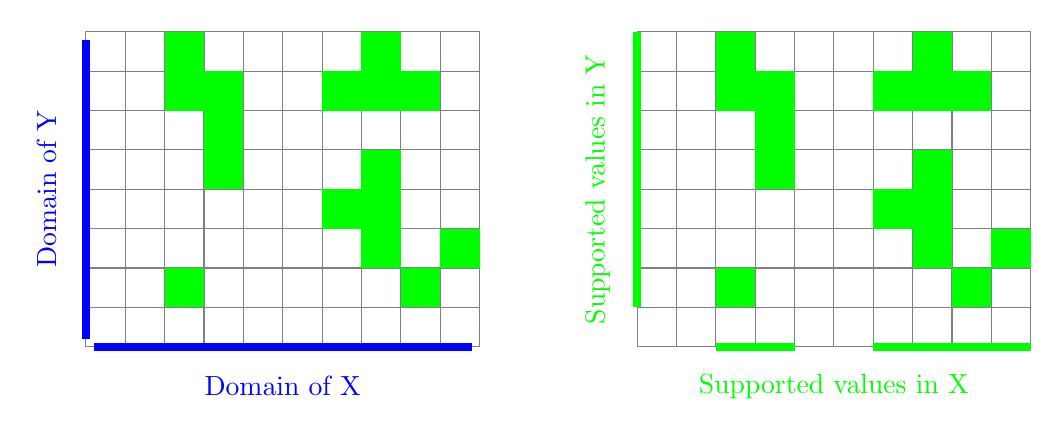
\begin{tikzpicture}
    \def\size{0.5}
    \def\columns{10}
    \pgfmathtruncatemacro{\lastCol}{\columns - 1}
    \def\rows{8}
    \pgfmathtruncatemacro{\lastRow}{\rows - 1}

    \foreach \x in {0,...,\lastCol} {
        \foreach \y in {0,...,\lastRow} {
            \draw[gray] 
            ({\x * \size}, {\y * \size})
            rectangle ++(\size,\size);
        }
    }
    
    % Row 2
    \foreach \x in {2,8} {
        \fill[green]
            ({\x * \size},{1 * \size})
            rectangle ++(\size,\size);
    }
    
    % Row 3
    \foreach \x in {7,9} {
        \fill[green]
            ({\x * \size},{2 * \size})
            rectangle ++(\size,\size);
    }
    
    % Row 4
    \foreach \x in {6,7} {
        \fill[green]
            ({\x * \size},{3 * \size})
            rectangle ++(\size,\size);
    }
    
    % Row 5
    \foreach \x in {3,7} {
        \fill[green]
            ({\x * \size},{4 * \size})
            rectangle ++(\size,\size);
    }

    % Row 6
    \fill[green]
        ({3 * \size},{5 * \size})
        rectangle ++(\size,\size);
    
    % Row 7
    \foreach \x in {2,3,6,7,8} {
        \fill[green]
            ({\x * \size},{6 * \size})
            rectangle ++(\size,\size);
    }

    % Row 8
    \foreach \x in {2,7} {
        \fill[green]
            ({\x * \size},{7 * \size})
            rectangle ++(\size,\size);
    }

    % Bottom border
    \node[text=blue] at ({(10*\size)/2}, -0.5) {Domain of X};
    \draw[line width=3pt, blue]
        (0.2 * \size, 0)
        -- ++(9.6 * \size, 0);

    % Left border
    \node[text=blue, rotate=90] at (-0.5, {(8*\size)/2}) {Domain of Y};
    \draw[line width=3pt, blue]
        (0, 0.2 * \size)
        -- ++(0, 7.6 * \size);
    
    \begin{scope}[shift={({\columns*\size + 2}, 0)}]
        \foreach \x in {0,...,\lastCol} {
            \foreach \y in {0,...,\lastRow} {
                \draw[gray] 
                ({\x * \size}, {\y * \size})
                rectangle ++(\size,\size);
            }
        }

        % Row 2
        \foreach \x in {2,8} {
            \fill[green]
                ({\x * \size},{1 * \size})
                rectangle ++(\size,\size);
        }
        
        % Row 3
        \foreach \x in {7,9} {
            \fill[green]
                ({\x * \size},{2 * \size})
                rectangle ++(\size,\size);
        }
        
        % Row 4
        \foreach \x in {6,7} {
            \fill[green]
                ({\x * \size},{3 * \size})
                rectangle ++(\size,\size);
        }
        
        % Row 5
        \foreach \x in {3,7} {
            \fill[green]
                ({\x * \size},{4 * \size})
                rectangle ++(\size,\size);
        }

        % Row 6
        \fill[green]
            ({3 * \size},{5 * \size})
            rectangle ++(\size,\size);
        
        % Row 7
        \foreach \x in {2,3,6,7,8} {
            \fill[green]
                ({\x * \size},{6 * \size})
                rectangle ++(\size,\size);
        }

        % Row 8
        \foreach \x in {2,7} {
            \fill[green]
                ({\x * \size},{7 * \size})
                rectangle ++(\size,\size);
        }

        % Bottom border
        \node[text=green] at ({(10*\size)/2}, -0.5) {Supported values in X};
        \draw[line width=3pt, green]
            (2 * \size, 0)
            -- ++(2 * \size, 0);
        \draw[line width=3pt, green]
            (6 * \size, 0)
            -- ++(4 * \size, 0);

        % Left border
        \node[text=green, rotate=90] at (-0.5, {(8*\size)/2}) {Supported values in Y};
        \draw[line width=3pt, green]
            (0, 1 * \size)
            -- ++(0, 7 * \size);
    \end{scope}
\end{tikzpicture}